\chapter{How to Do a Search}

In a particle physics search, we hypothesize the existence of a previously undetected particle or interaction, and we perform statistical analysis on our collision data to try to find evidence for it. A search is usually considered successful when we see a likelihood z-score of 5 or greater, as will be explained shortly.

\subsection*{Models, Regions, and Backgrounds}

The first step of a search is to draw up a model for a specific decay process which could exist. For example, the ATLAS Higgs search considered the decay process $H\rightarrow ZZ^*\rightarrow 4\ell$, in which a Higgs boson decays to a final state with four leptons~\cite{HiggsATLAS}. In this hypothesis, the process would exist on top of the known Standard Model processes, involving the production and decay of known particles in known ratios (given the beam center-of-mass energy).

Next, we define a search region by placing requirements on our objects and events. This is done to maximize the ratio of signal events over background events. For the Higgs analysis, the authors looked at regions with four leptons, composed of two opposite-sign same-flavor lepton pairs. The invariant masses of these leptons were also required to fall within certain ranges. This is on top of lepton reconstruction requirements, such as isolation, energy, and angle cuts~\cite{HiggsATLAS}.

After the region is selected, we then consider which Standard Model processes would contribute to the background events in this region. The bulk of the search then entails methods of estimating these background contributions, as well as placing uncertainties on them. The background estimation methods are typically developed and validated with Monte Carlo events.

After that, the methods are checked in data validation regions, which are defined to be orthogonal to our signal regions. In other words, the validation regions have no events in common with the regions we are actually interested in, to prevent any knowledge of our results from leaking into the method development process. Validation regions are often similar to signal regions, but with a single shifted requirement. For example, instead of requiring \MET\ from 100 to 200 GeV, the validation region may require 200 to 300 GeV.

We are not allowed to look at (i.e. unblind) our signal regions until all methods have been developed and validated, and approval has been given by a centralized board after peer review.

\subsection*{Uncertainties}

After the background estimation techniques are developed, we then have to carefully consider the uncertainties in these estimated yields. There are two kinds of uncertainties - statistical and systematic.

Statistical uncertainties come about due to the randomness inherent in observing a stochastic process. For example, if we observe that a certain number of events pass our signal region, we can place a standard deviation on that observation which would reflect the fluctuations we expect to see if we ran the entire ATLAS experiment over again from the beginning.

Systematic uncertainties, on the other hand, reflect uncertainties in yield due to weaknesses in our estimation methods. For example, MC generators are not perfect, and have to rely on effective parameters for modelling of some computationally intractable interactions. If these parameters are set high or low within a range, we can get smaller or larger yields. This yield range can be used as a systematic uncertainty. There may also be components of our estimation methods that require taking ratios of event yields in certain regions, e.g. for scaling purposes. The statistical uncertainties in these yields would then produce systematic uncertainties in our methods.

\subsection*{Results and Plots}

Once we unblind our data, we are able to compare data yields in our signal regions vs. expected yields for the Standard Model backgrounds. From this we can calculate probabilities for the existence of our signal processes.

In high energy analyses we prefer to use frequentist approaches, to avoid the priors required in Bayesian approaches. Often we are interested in drawing exclusion curves, to mark out parts of the model parameter space where the likelihood of those models given the observed data is less than some percentage.

To avoid the situation where a downward statistical fluctuation in an observation could actually exclude the Standard Model, we don't use a standard likelihood measure. Rather, we often use something called $CL_s$~\cite{CLs}, where we take the ratio of likelihoods for the Standard Model plus signal process ($H_1$), vs. just the Standard Model ($H_0$).

In practice, to draw exclusion curves we usually produce a grid of signal models with different model parameters. We call these toy MC models. For each point on this grid, we compute the $CL_s$ for the model with those parameters. This allows us to draw plots like the Brazil-band plot~\cite{Brazil_band} in Figure~\ref{fig:Higgs_CLs}, for the Higgs boson discovery in ATLAS~\cite{HiggsATLAS}.

This plot shows both the expected exclusion curve and the observed exclusion curve. The expected curve shows which parts of the parameter space would be excluded if we obtained yields according to the non-Higgs Standard Model background. The dashed line shows the mean expected background exclusion, and the green and yellow bands show one and two standard deviations. That is, at the top edge of the yellow band, those parameter space points would be excluded at about $5\%$ if we were to see a non-Higgs SM expected yield. The solid line shows which parts of the parameter space would be excluded using actual observed data.

\begin{figure}[htbp]
    \centering
    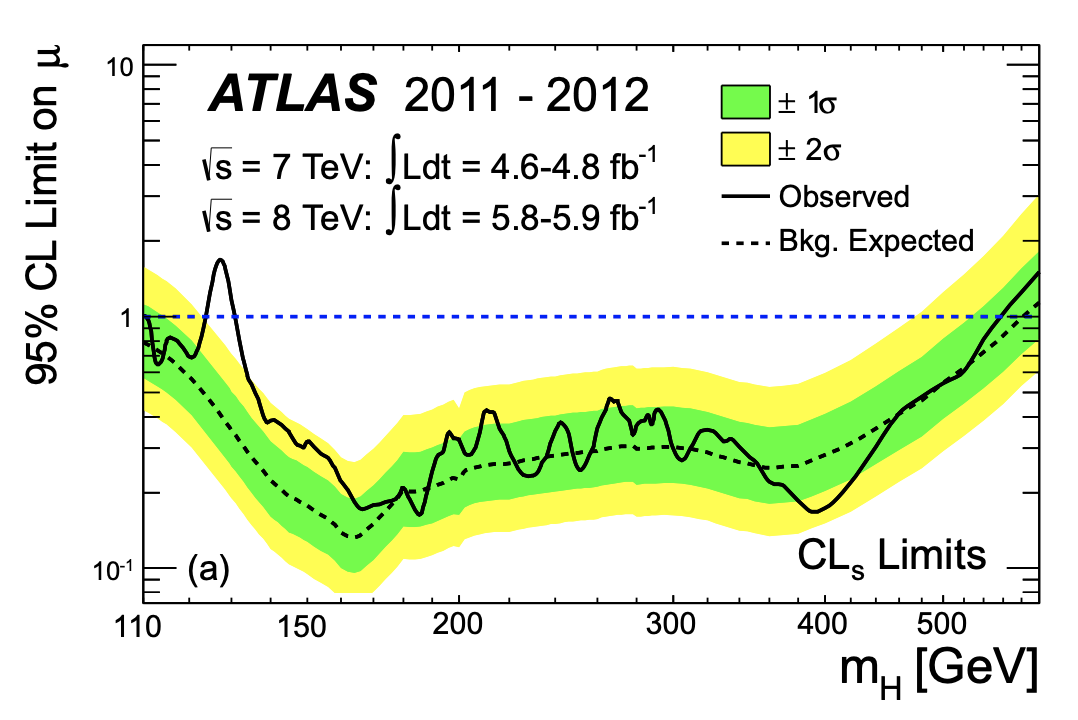
\includegraphics[width=\linewidth]{Images/ATLAS/Higgs_CLs.png}
    \caption{The model parameter space here is over the Higgs mass and a scale factor $\mu$ on the Higgs cross section. The region above the curve is excluded. The dashed line represents the exclusion based only on the expected (non-Higgs) SM background, while the solid line is based on observed data. Standard Model Higgs are excluded when the solid line is below $\mu<1$. The solid line is above both the dashed line and $\mu=1$ at $m_H=126$, indicating both that a SM Higgs is not excluded at this mass, and that the observation at this point far exceeds what one is likely to see from a non-Higgs background. Figure from~\cite{HiggsATLAS}.}
    \label{fig:Higgs_CLs}
\end{figure}